\documentclass[xcolor=table, aspectratio=169, bigger]{beamer}

\usepackage{shyne}

% Theme settings
\setbeamertemplate{navigation symbols}{}

\usetheme{Madrid}
\usefonttheme{structurebold}
\usefonttheme[onlymath]{serif}

\AtBeginSection[]
{ 	\begin{frame}{}

	{
	\usebeamerfont{frametitle}
	\begin{beamercolorbox}
		[wd={\textwidth}, center, sep=.2in, rounded=true, shadow=true]
		{frametitle}
	Week \thesection\\  \secname 
	\end{beamercolorbox}
	}
	
	\end{frame} 
}

\AtBeginSubsection[]
{ 	\begin{frame}{}

	{
	\usebeamerfont{frametitle}
	\begin{beamercolorbox}
		[wd={\textwidth}, center, sep=.2in, rounded=true, shadow=true]
		{frametitle}
	Section \thesection .\thesubsection\\  \subsecname 
	\end{beamercolorbox}
	}
	
	\end{frame} 
}

\title[Week 8]{Stat 201: Statistics I\\Week 9 }
\author[M. Shyne]{}
\institute[Metro State]{
\includegraphics[width=1.75in]{../images/metro_logo}}
\date[3/30/2019]{
\\ \bigskip \bigskip 
\includegraphics[width=.4in]{../images/cc_big}}



\begin{document}
\frame{\titlepage}

% Week 9
\setcounter{section}{8}
\section{Inference for Numerical Data}

%
% Section 9.1
%
\subsection{One sample hypothesis tests for means}


%%%%%%%%%%
\begin{frame}{Student's t distribution}

\begin{block}{}
Recall, the Central Limit Theorem states that, under the right conditions, a sampling distribution is normally distributed with a standard error defined by the population standard deviation. However, when the population standard deviation is unknown, it must be estimated by the sample standard deviation.
\end{block}

\pause
\begin{block}{}
\bt{Student's t distribution} is similar to a normal distribution, except with an adjusted shape to account for an estimated standard deviation.\\
\begin{itemize}
\pause\item The $t$ distribution has an added parameter known as the degrees of freedom (df).
\pause\item The degrees of freedom for a sampling distribution is defined as sample size minus one ($df = n-1$).
\pause\item As degrees of freedom increases, the $t$ distribution approaches a normal distribution.
\end{itemize} 
\end{block}
\end{frame}

%%%%%%%%%%
\begin{frame}{Student's t distribution}
\medskip
{\centering
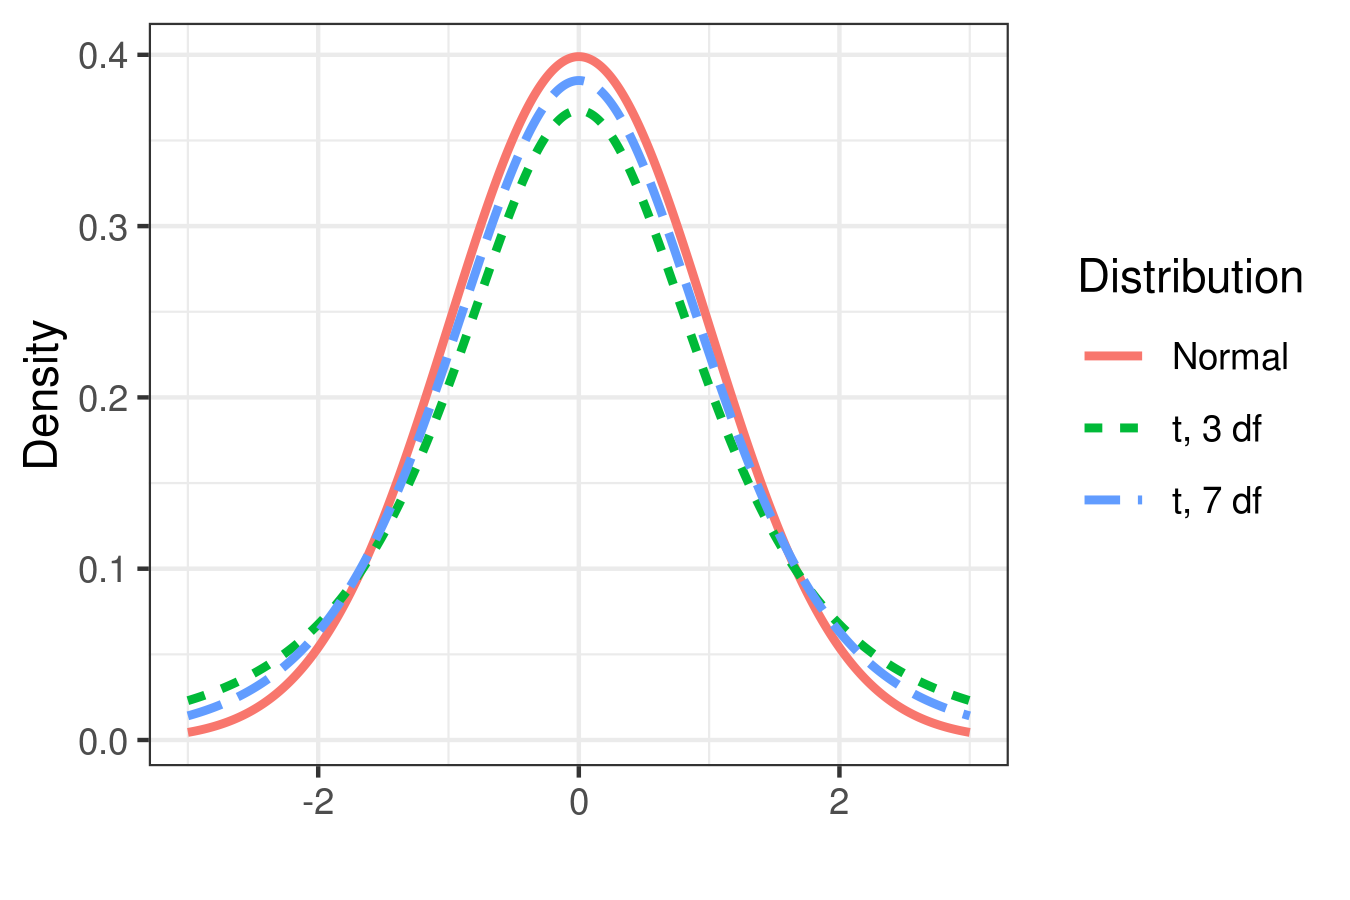
\includegraphics[width=4.5in]{../images/wk09_t_dist}
\par}
\end{frame}

%%%%%%%%%%
\begin{frame}{Steps for a mean hypothesis test}
\begin{block}{}
\begin{enumerate}
\item Identify null and alternative hypotheses from research question\\
$H_0: \mu = \mu_0$\\
$H_a: \mu \ne \mu_0, \, \mu < \mu_0, \, \mu> \mu_0$
\item Use a t distribution
\item Calculate $t$ test statistic
\item Calculate p-value
\item Compare p-value to significance level $\alpha$ and report decision
\item State conclusion in terms of original research question
\end{enumerate}
\end{block}
\end{frame}


%%%%%%%%%%
\begin{frame}{Test statistic for mean tests}
\begin{block}{}
Tests for population means use the t sampling distribution. The test statistic is a $t$-score.
\[t = \frac {\bar x - \mu_0}{s/\sqrt{n}}\]
where $\bar x$ is the sample mean, $\mu_0$ is the population mean under the null hypothesis, $s$ is the sample standard deviation and $n$ is the sample size.
\end{block}

\end{frame}


%%%%%%%%%%
\begin{frame}{p-values for mean tests}
\begin{block}{}
Given a $t$ test statistic, the p-value is the probability of getting $t$-scores more extreme on a t distribution.
\begin{itemize}
\pause\item For two-sided test:\\ 
$H_a: \mu \ne \mu_0$, p-value = $P(T<-t) + P(T > t) = \begin{cases}2 \times P(T > t), & t >0 \\ 2 \times P(T<t), & t < 0\end{cases}$
\pause\item For one-sided test:\\
$H_a: \mu < \mu_0$, p-value = $P(T < t)$\\
$H_a: \mu > \mu_0$, p-value = $P(T > t)$
\end{itemize}
\end{block}
\end{frame}




%%%%%%%%%%
\begin{frame}{Hypothesis test for a mean, example}
\begin{exampleblock}{Example}
A study is conducted of the heights of Metro State students. The heights of a sample of 35 male students are measured. The mean height from the sample is $\bar x = 68.1$ with a standard deviation of $s=3.5$. Conduct a test at $\alpha=0.05$ level of significance of the claim that male Metro State students are shorter than the general population of 69.2 inches.
\begin{enumerate}
\pause\item Identify null and alternative hypotheses from research question\\
\pause$H_0: \mu = 69.2$\\
$H_a: \mu < 69.2$\\
Population: Male Metro State students
\end{enumerate}
\end{exampleblock}
\end{frame}

%%%%%%%%%%
\begin{frame}{Hypothesis test for a mean, example}
\begin{exampleblock}{Example}
\begin{enumerate}
\setcounter{enumi}{1}

\item Use a t distribution
\pause\item Calculate $t$ test statistic\\
\pause\smallskip$\ds t=\frac{\bar x - \mu_0}{s / \sqrt{n}} = \frac{68.1 - 69.2}{3.5 / \sqrt{35}} = -1.859339$
\pause\item Calculate p-value\\
\pause$p = P(T < t) = P(T < -1.859) = 0.0358$
\pause\item Compare p-value to significance level $\alpha$ and report decision\\
\pause$p = 0.0358 < \alpha = 0.05$. Reject the null hypothesis.
\pause\item State conclusion in terms of original research question\\
\pause There is evidence that male Metro State students are shorter than the general population.
\end{enumerate}

\end{exampleblock}
\end{frame}

%%%%%%%%%%
\begin{frame}{Hypothesis test for a mean, example}
\begin{exampleblock}{Example}
A clinical trial of an experimental drug for a rare disease is conducted. The survival times in months of 10 patients given the new drug are below. Test the claim that the drug changes the survival time for the expected survival time of 36 months at a 0.01 level of significance.\\
\medskip
{\centering
35.5, 40.5, 44.7, 37.2, 34.7, 41.3, 37.8, 34.5, 39.8, 37.1
\par}
\begin{enumerate}
\pause\item Identify null and alternative hypotheses from research question\\
\pause$H_0: \mu = 36$\\
$H_a: \mu \ne 36$\\
Population: Patients with disease taking experiment drug
\end{enumerate}
\end{exampleblock}
\end{frame}

%%%%%%%%%%
\begin{frame}{Hypothesis test for a mean, example}
\begin{exampleblock}{Example}
\begin{enumerate}
\setcounter{enumi}{1}

\item Use a t distribution
\pause\item Calculate $t$ test statistic\\
\pause$t=2.2462$
\pause\item Calculate p-value\\
\pause$p = 0.05132$
\pause\item Compare p-value to significance level $\alpha$ and report decision\\
\pause$p = 0.05132 > \alpha = 0.01$. Do not reject the null hypothesis.
\pause\item State conclusion in terms of original research question\\
\pause There is not evidence that the experimental drug changes survival time.
\end{enumerate}

\end{exampleblock}
\end{frame}

%%%%%%%%%%
%%%%%%%%%%
\begin{frame}<handout:0>{Group work}
\begin{block}{}
\large
\begin{itemize}
\item Complete question 1.
\end{itemize}
\end{block}
\end{frame}

%
% Section 9.2
%
\subsection{Two sample hypothesis tests for means}

%%%%%%%%%%
\begin{frame}{Two sample hypothesis testing}
\begin{block}{}
Previously, a single sample was used to test whether the population from which the sample was drawn was the same or similar to a known population. More precisely, an hypothesis test compares an unknown population parameter to a known value.\\
\pause\medskip
Hypothesis testing can be used to compare two unknown populations using samples drawn from each population. This is unsurprisingly known as \bt{two sample hypothesis testing}. These tests compare two unknown population parameters.
\end{block}
\end{frame}

%%%%%%%%%%
\begin{frame}{Null hypotheses}
\begin{block}{}
The null hypothesis is the claim that nothing interesting has occurred. For one sample tests, the null hypothesis states that the unknown population parameter is the same as the known parameter or some other known value.\\
\medskip
\pause For two sample tests, the null hypothesis states that the two unknown parameters are the same.\\
\medskip
\pause For example, if comparing means, $H_0: \mu_1 = \mu_2$, or the mean of population 1 is the same as the mean of population 2.
\end{block}
\end{frame}

%%%%%%%%%%
\begin{frame}{Alternative hypotheses}
\begin{block}{}
The alternative hypothesis is then the claim that something interesting has occurred. For one sample tests, the alternative hypothesis states that the unknown population parameter is somehow different from the known parameter. The unknown parameter might be less than, greater than or simple not equal to the known value. \\
\pause\medskip
For two sample tests, the alternative hypothesis states that the two unknown parameters are different. Similar to a one sample test, the alternative hypothesis could state that the first population parameter is less than, greater than or not equal to the second population parameter.\\
\pause\medskip
For example, if comparing means, $H_a: \mu_1 < \mu_2$ or $\mu_1 > \mu_2$ or $\mu_1 \ne \mu_2$.
\end{block}
\end{frame}

%%%%%%%%%%
\begin{frame}{Conducting two sample hypothesis test}
\begin{block}{}
Once the null and alternative hypotheses are determined, two sample hypothesis tests are carried out almost identically to one sample hypothesis tests.\\
\medskip
Assuming the null hypothesis is true, a test statistic representing the place of the samples within the appropriate sampling distribution is calculated. A p-value representing the probability of obtaining the test statistic or one more extreme is calculated. If the p-value is below a pre-determined threshold (the significance level), then the null hypothesis is rejected and it can be said that there is evidence for the alternative hypothesis.
\end{block}
\end{frame}


%%%%%%%%%%
\begin{frame}{Independent vs. dependent samples}
\begin{block}{}
Before conducting a test, it must be determined whether the samples are independent or dependent.\\
\pause\medskip
\bt{Independent samples} are samples that come from distinct populations where the values from one sample do not affect the values from the other samples.\\
\pause\medskip
Conversely, \bt{dependent samples} are samples that often involve the same subjects with measurements taken at different times.
\end{block}
\end{frame}

%%%%%%%%%%
\begin{frame}{Independent vs dependent samples, example}
\begin{exampleblock}{Example}
Independent samples:
\begin{itemize}
\item Scores on statistic final in one class vs another class
\item Heights of men vs heights of women
\item In a clinical trial, outcomes for patients given experiment treatment vs patients given placebo (control)
\end{itemize}
\pause
Dependent samples:
\begin{itemize}
\item Scores on midterm exam vs final exam
\item Heights of husbands vs heights of wives
\item In a case control study, risk factors for subjects with disease vs matched subjects without disease
\end{itemize}
\end{exampleblock}
\end{frame}

%%%%%%%%%%
\begin{frame}{Null and alternative hypotheses, independent samples}
\begin{block}{}
The null hypothesis for two sample mean tests is always $H_0: \mu_1 = \mu_2$ or $H_0: \mu_1 -\mu_2 = 0$.\\
\medskip
Alternative hypotheses can be any of\\
\medskip
\eq{ H_a: \mu_1 < \mu_2, \, \mu_1 > \mu_2, \, \mu_1 \ne \mu_2}
\medskip
 or the equivalent forms of \\
 \medskip
{\centering $H_a: \mu_1 - \mu_2 < 0, \, \mu_1 - \mu_2 > 0, \, \mu_1 - \mu_2 \ne 0$ \par}
\medskip

\end{block}
\end{frame}

%%%%%%%%%%
\begin{frame}{Requirements}
\begin{block}{}
Both samples must be independent and simple random samples drawn from normal populations or have a sample size of at least 30.
\end{block}
\end{frame}

%%%%%%%%%%
\begin{frame}{Test statistic}
\begin{block}{}
As with one sample mean tests, two sample mean tests use a t distribution. Similar to two sample proportion tests, a t statistic  is calculated by\\
\medskip
\eq{t = \frac {\bar x_1 - \bar x_2}{\sqrt{\frac{s_1^2}{n_1} + \frac{s_2^2}{n_2}}}}
\medskip\pause
Recall, the degrees of freedom of a t distribution is defined by sample size minus one ($n-1$). For a two sample test, a conservative approach is to use the smaller of the degrees of freedom from the two samples.\\
\medskip
{\centering $\ds df = \min\Brack{(n_1-1) , (n_2-1)}$ \par}
\pause\medskip
When using technology, a more complicated, but accurate value will be used for the degrees of freedom.
\end{block}
\end{frame}


%%%%%%%%%%
\begin{frame}{Hypothesis test for two means, example}
\begin{exampleblock}{Example}
A study is conducted of the heights of Metro State students. The heights of a sample of 32 male students taking statistics (population 1) have a mean of $\bar x = 70.1$ with a standard deviation of $s=3.5$. The heights of a sample of 38 male students taking accounting (population 2) have a mean of $\bar x = 67.9$ with a standard deviation of $s=3.1$.\\
\medskip
Conduct a test at $\alpha=0.05$ level of significance of the claim that statistics students are taller than accounting students.
\begin{enumerate}
\pause\item Identify null and alternative hypotheses from research question\\
\pause$H_0: \mu_1 = \mu_2$ of $H_0: \mu_1 - \mu_2 = 0$\\
$H_a: \mu_1 > \mu_2$ or $H_a: \mu_1 - \mu_2 > 0$\\
\end{enumerate}
\end{exampleblock}
\end{frame}

%%%%%%%%%%
\begin{frame}{Hypothesis test for two means, example}
\begin{exampleblock}{Example}
\begin{enumerate}
\setcounter{enumi}{1}

\item Use a t distribution
\pause\item Calculate $t$ test statistic\\ \medskip
\pause$\ds t = \frac {\bar x_1 - \bar x_2}{\sqrt{\frac{s_1^2}{n_1} + \frac{s_2^2}{n_2}}} = \frac {70.1 - 67.9}{\sqrt{\frac{3.5^2}{32} + \frac{3.1^2}{38}}} = 2.759269$
\pause\item Calculate p-value\\
\pause$p = P(T > t) = P(T > 2.759) = 0.0048$
\pause\item Compare p-value to significance level $\alpha$ and report decision\\
\pause$p = 0.0048 < \alpha = 0.05$. Reject the null hypothesis.
\pause\item State conclusion in terms of original research question\\
\pause There is evidence that male statistics students are taller than male accounting students.
\end{enumerate}

\end{exampleblock}
\end{frame}


%%%%%%%%%%
\begin{frame}{Hypothesis tests for dependent samples}
\begin{block}{}
Conceptually, when working with two dependent samples, also known as matched pairs, a new value $d = x_1 - x_2$ is calculated for each pair. Then, the null hypothesis $H_0: \mu_1 = \mu_2$ becomes $H_0: \mu_D = 0$ and the test is essentially a one sample hypothesis test for the mean of $d$.\\
\pause\medskip
Matched pairs tests, when appropriate, are preferable to independent samples tests because the variability between subjects is almost eliminated. Thus, the total variability is reduced resulting in a more accurate test. 
\end{block}
\end{frame}

%%%%%%%%%%
\begin{frame}{Conducting a dependent samples test}
\begin{block}{}
Since a dependent samples test is essentially a one sample test of the sample of difference values $d$, null and alternative hypotheses should be stated in terms of $\mu_D$ the population mean of the differences.\\
\pause\medskip
For example, $H_0: \mu_D = 0$ and $H_a: \mu_D < 0$.\\
\pause\medskip
The test statistic is calculated as a one sample statistic from the sample of differences\\
\medskip
{\centering $\ds t = \frac {\bar d}{\frac{s_d}{\sqrt{n}}}$ \par}
\medskip
\end{block}
\end{frame}



%%%%%%%%%%
\begin{frame}{Hypothesis test for matched pairs, example}
\begin{exampleblock}{Example}
A study is conducted to see if statistics students change their scores from the midterm exam to the final exam. 42 students who took both exams are randomly selected. Their scores are found in the file ``scores.csv".\\
\medskip
Test at significance level of 0.01 whether scores changed between the midterm and the final.
\begin{enumerate}
\pause\item Identify null and alternative hypotheses from research question\\
\pause$H_0: \mu_D = 0$\\
$H_a: \mu_D \ne 0$\\
\end{enumerate}
\end{exampleblock}
\end{frame}

%%%%%%%%%%
\begin{frame}{Hypothesis test for matched pairs, example}
\begin{exampleblock}{Example}
\begin{enumerate}
\setcounter{enumi}{1}

\item Use a t distribution
\pause\item Calculate $t$ test statistic\\
\pause$t=-3.8176772$
\pause\item Calculate p-value\\
\pause$p = 0.0004$
\pause\item Compare p-value to significance level $\alpha$ and report decision\\
\pause$p = 0.0004 < \alpha = 0.01$. Reject the null hypothesis.
\pause\item State conclusion in terms of original research question\\
\pause There is evidence that statistics exam scores change from the midterm to the final.
\end{enumerate}

\end{exampleblock}
\end{frame}


%%%%%%%%%%
\begin{frame}<handout:0>{Group work}
\begin{block}{}
\large
\begin{itemize}
\item Complete questions 2 and 3.
\end{itemize}
\end{block}
\end{frame}


%%%%%%%%%%
\begin{frame}{Teaching the null hypothesis}
\smallskip
{\centering

\includegraphics[width=1.8 in]{../images/ch09_null_hypothesis}
\par}
\end{frame}

\end{document}